\documentclass[landscape, 8pt, a4paper]{extarticle}
\usepackage[ngerman]{babel}
\usepackage[utf8]{inputenc}
\usepackage{lmodern}
\usepackage[T1]{fontenc}
\renewcommand{\familydefault}{\sfdefault}

\usepackage{amsmath}
\usepackage[fleqn]{mathtools}
\usepackage{amssymb}
\usepackage{amsfonts}
\usepackage{latexsym}
\usepackage[landscape, margin=1cm]{geometry}
\usepackage{enumitem}
\usepackage{multicol}
\usepackage{fancyhdr}



\pagestyle{empty}

\setlength{\parindent}{0pt}


\setlist[2]{noitemsep}
\setitemize{noitemsep, leftmargin=8pt, itemindent=0pt, labelsep=3pt, labelwidth=0pt, labelindent=0pt}
\setlength{\belowdisplayskip}{0pt} \setlength{\belowdisplayshortskip}{0pt}
\setlength{\abovedisplayskip}{0pt} \setlength{\abovedisplayshortskip}{0pt}

\newcommand{\poly}{\textbf{P}}
\newcommand{\npoly}{\textbf{NP}}
\newcommand{\N}{\mathbb{N}}
\newcommand{\set}[2]{\ensuremath\left\{ #1 \,\middle|\, #2 \right\}}
\newcommand{\simpleset}[1]{\ensuremath\left\{ #1 \right\}}

\begin{document}
\begin{multicols}{3}
	\textbf{Simon König 3344789 - Klausurzettel}

	Turingmaschine: $M=(Z,\Sigma,\Gamma,\delta,z_0,\Box,E)$ mit $\delta: Z\times\Gamma\rightarrow Z\times\Gamma\times\simpleset{L,N,R}$

	ATM: zusätzlich $t: Z\rightarrow \simpleset{\forall, \exists}$

	Endl. Automat: $M=(Z,\Sigma, \delta, S, E)$

	Gerich. Graph $G=(V,E), E= \set{(v,w)\in V^2}{\text{von $v$ zu $w$}}$

	Unger. Graph $G=(V,E), E= \set{\simpleset{v,w}\subseteq V}{\text{$v,w$ sind verbunden}}$

	\section{Berechenbarkeit}
	\begin{itemize}
		\item \textbf{LOOP-Anweisungen}:
		\begin{itemize}
			\item $x_i\coloneqq x_j+c$ bzw. $x_i\coloneqq x_j-c$ mit $c\in\N$
			\item \texttt{LOOP} $x_i$ \texttt{DO} $P$ \texttt{END}
			\item Hintereinanderausführung von LOOP-Programmen
		\end{itemize}

		\item \textbf{Primitiv rekursive Funktionen}:
		\begin{multicols}{2}
			\begin{itemize}
				\item \texttt{s(n)}
				\item \texttt{dec(n)}
				\item \texttt{add(a,b)}
				\item \texttt{sub(a,b)}
				\item \texttt{mul(a,b)}
				\item \texttt{c$^i_j$=j}
				\item \texttt{even(n)}
				\item \texttt{odd(n)}
				\item \texttt{leq(a,b)}
				\item \texttt{eq(a,b)}
				\item \texttt{c(x,y)}
			\end{itemize}
		\end{multicols}

		\item \textbf{Turing-berechenbar (nicht LOOP)}:
		\begin{itemize}
			\item $\Omega$, nirgends definierte Funktion
			\item $a(x,y)$, Ackermannfunktion
		\end{itemize}

		\item \textbf{$\mu$-Rekursion bzw. WHILE}:
		\begin{itemize}
			\item Für eine Funktion $f(x_1,x_2,\ldots,x_k)$ ist
			\begin{align*}
				\mu f(x_2,\ldots,x_k)=\min\{n\in\N | &f(n,x_2,\ldots,x_k)=0\\&\wedge f(n_0,x_2,\ldots,x_k)>0 \enspace\forall n_0<n\}
			\end{align*}
			\item \textbf{Satz von Kleene}: Jede WHILE-berechenbare Funktion lässt sich mit einer WHILE-Schleife darstellen. Genauso bei $\mu$-Rekursion mit einem $\mu$-Operator.
		\end{itemize}
	\end{itemize}

	\section{Entscheidbarkeit}
	\begin{itemize}
		\item $A\leq B$ und $A$ \textit{nicht} semi-entscheidbar, dann ist $B$ ebenfalls nicht semi-entscheidbar.
		Ist $B$ semi-entscheidbar, dann ist auch $A$ semi-entscheidbar.
		\item \textbf{Dovetailing}:
		Simuliere Maschine $M$ auf Eingabe $\omega(e(n))$ genau $f(n)$ Schritte lang, erhöhe $n$. Hierbei sei $\omega(n)$ die Funktion zur rekursiven Aufzählbarkeit. $e(c(a,b))=a$ und $f(c(a,b))=b$.
		\item \textbf{Satz von Rice}: $\mathcal R$ die Menge der Turing-berechenbaren Funktionen. Die Menge
		\begin{equation*}
			\mathcal C(\mathcal S)=\set{w}{M_w\text{ berechnet eine Funktion aus } \mathcal S}
		\end{equation*}
		ist unentscheidbar, wenn $\emptyset\neq\mathcal S\neq\mathcal R$.
		\item Eine Sprache ist genau dann semi-entscheidbar, wenn sie sich auf $H$ reduzieren lässt. (Vortragsübung)
		\item Für zwei kontextfreie Grammatiken sind unentscheidbar: Leerheit des Schnitts, Endlichkeit des Schnitts, Kontextfreiheit des Schnitts, Inklusion und Äquivalenz

		\item \textbf{Entscheidbarkeiten}:

		\begin{tabular}{r|cccc}
			&Wortproblem&Leerheit&Äquivalenz&Schnitt\\
			REG&\checkmark&\checkmark&\checkmark&\checkmark\\
			DCFL&\checkmark&\checkmark&\checkmark&X\\
			CFL&\checkmark&\checkmark&X&X\\
			CSL&\checkmark&X&X&X\\
			r.e.&X&X&X&X
		\end{tabular}

		\item \textbf{Abschlusseigenschaften}:

		\begin{tabular}{r|ccccc}
			&Schnitt&Vereinig.&Kompl.&Konkat.&Stern\\
			REG&\checkmark&\checkmark&\checkmark&\checkmark&\checkmark\\
			DCFL&X&X&\checkmark&X&X\\
			CFL&X&\checkmark&X&\checkmark&\checkmark\\
			CSL&\checkmark&\checkmark&\checkmark&\checkmark&\checkmark\\
			r.e.&\checkmark&\checkmark&X&\checkmark&\checkmark
		\end{tabular}
	\end{itemize}


	\subsection{Entscheidbarkeitsprobleme}
	\begin{tabular}{r|c|l}
		Spez Haltep & $K=\set{w}{M_w \text{ hält auf Eingabe } w}$ & semi\\
		Allg Haltep & $H=\set{w\# x}{M_w \text{ hält auf Eingabe } x}$ & semi\\
		Haltep auf $\epsilon$ & $H_0=\set{w}{M_w \text{ hält auf Eingabe } \epsilon}$ & semi\\
		PCP & $((x_1,y_1),\ldots,(x_n,y_n))$ zusammenpassen & semi\\
		MPCP & Für alle Lösungen gilt $i_1=1$ & semi\\
		WA & Menge aller wahren arithm. Formeln & unentsch.\\
		$\overline{WA}$ & Menge aller falschen arithm. Formeln & unentsch.
	\end{tabular}

	\section{Komplexität}
	\begin{itemize}
		\item Wichtige Komplexitätsklassen \begin{itemize}
			\item $\textbf{PSPACE}=\bigcup \operatorname{DSPACE}(p)=\bigcup \operatorname{NSPACE}(p)$
			\item $\npoly = \bigcup \operatorname{NTIME}(p)$
			\item $\poly = \bigcup \operatorname{DTIME}(p)$
			\item $\textbf{NL}=\operatorname{NSPACE}(\log n)$
			\item $\textbf{L}=\operatorname{DSPACE}(\log n)$
		\end{itemize}
		\item $\operatorname{co}\mathcal C=\set{L}{\overline L\in \mathcal C}$ und $\overline{\mathcal C}=\set{L}{L\not \in \mathcal C}$
		\item In den Platzklassen ist $\mathcal O$-Notation egal, Konstanten können vernachlässigt werden
		\begin{align*}
			\operatorname{DSPACE}(\mathcal O(f))&=\operatorname{DSPACE}(f)\\
			\operatorname{NSPACE}(\mathcal O(f))&=\operatorname{NSPACE}(f)
		\end{align*}
		\item In nichtdeterministischen Zeitklassen spielt die $\mathcal O$-Notation keine Rolle
		\begin{equation*}
			\operatorname{NTIME}(\mathcal O(f))=\operatorname{NTIME}(f)
		\end{equation*}
		\item Bei deterministischen Zeitklassen gilt i.A. $\operatorname{DTIME}(\mathcal O(f))\not=\operatorname{DTIME}(f)$, nur für größer als lineare Funktionen gilt Gleichheit d.h.
		\begin{align*}
			\operatorname{DTIME}(\mathcal O(f))&=\operatorname{DTIME}(f) \enspace f(n)\geq (1+\epsilon)n\text{ für ein }\epsilon>0
		\end{align*}
		\item \textbf{Satz von Hennie und Stearns}: Falls $\epsilon>0, f(n)\geq (1+\epsilon)n$, dann gilt
		\begin{equation*}
			\operatorname{DTIME}(f)\subseteq\operatorname{DTIME}_{\text{2-Band}}(f\log f)
		\end{equation*}
		\item Für alle $f(n)\geq n$ gilt für die Zeitklassen
		\begin{equation*}
			\operatorname{DTIME}(f)\subseteq\operatorname{NTIME}(f)\subseteq\operatorname{DSPACE}(f)
		\end{equation*}
		\item Und für alle $f(n)\geq \log n$ gilt
		\begin{equation*}
			\operatorname{DSPACE}(f)\subseteq\operatorname{NSPACE}(f)\subseteq\operatorname{DTIME}(2^{\mathcal O(f)})
		\end{equation*}
		\item \textbf{Satz von Immerman und Szelepcsenyi}: Falls $f\in \Omega(\log(n))$, gilt:
		\begin{equation*}
			\operatorname{NSPACE}(f)=\operatorname{coNSPACE}(f)
		\end{equation*}
		\item Alle deterministischen Zeit- und Platzklassen sind gegen Komplement abgeschlossen:
		\begin{gather*}
			\operatorname{DSPACE}(f)=\operatorname{coDSPACE}(f)\\
			\operatorname{DTIME}(f)=\operatorname{coDTIME}(f)
		\end{gather*}
		\item \textbf{Satz von Savitch}: Sei $s\in\Omega(\log(n))$, dann gilt
		\begin{equation*}
			\operatorname{NSPACE}(s)\subseteq\operatorname{DSPACE}(s^2)
		\end{equation*}
		\item Sei $s_1\not\in\Omega(s_2)$ und $s_2\in\Omega(\log(n))$ und beide platzkonstruierbar, dann gilt der \textbf{Platzhierarchiesatz}
		\begin{gather*}
			\operatorname{DSPACE}(s_2)\setminus\operatorname{DSPACE}(s_1)\not=\emptyset\\
			\Rightarrow \operatorname{DSPACE}(s_1)\subsetneq\operatorname{DSPACE}(s_2)
		\end{gather*}
		\item Sei $t_1\log(t_1)\not\in\Omega(t_2)$ und $t_2\in\Omega(n\log(n))$ und beide zeitkonstruierbar, dann gilt der \textbf{Zeithierarchiesatz}
		\begin{gather*}
			\operatorname{DTIME}(t_2)\setminus\operatorname{DTIME}(t_1)\not=\emptyset\\
			\Rightarrow \operatorname{DTIME}(t_1)\subsetneq \operatorname{DTIME}(t_2)
		\end{gather*}
		\item \textbf{Lückensatz von Borodin}: Für jede totale berechenbare Funktion $r(n)\geq n$ existiert effektiv eine totale berechenbare Funktion $s(n)\geq n+1$ mit
		\begin{equation*}
			\operatorname{DTIME}(s(n))=\operatorname{DTIME}(r(s(n)))
		\end{equation*}
		\item Translationtechnik:\\
		Die Translationssätze werden verwendet, Separationen von größeren zu kleineren Klassen bzw. Gleichheiten oder Inklusionen von kleineren zu größeren Klassen zu übertragen.
		Die durch Padding aufgebläte Sprache ist $Pad_f(L)\coloneqq \set{w\$^{f(|w|)-|w|}}{w\in L}$.
		\begin{enumerate}
			\item Für zwei Funktionen $f(n),g(n)\geq n$ gilt der \textbf{Translationssatz für Zeitklassen}:
			\begin{align*}
				Pad_f(L)\in \operatorname{DTIME}(\mathcal O(g))&\Leftrightarrow L\in \operatorname{DTIME}(\mathcal O(g\circ f))\\
				Pad_f(L)\in \operatorname{NTIME}(\mathcal O(g))&\Leftrightarrow L\in \operatorname{NTIME}(\mathcal O(g\circ f))
			\end{align*}
			\item Und analog für $g\in\Omega(\log)$ und $f(n)\geq n$ der \textbf{Translationssatz für Platzklassen}:
			\begin{align*}
				Pad_f(L)\in \operatorname{DSPACE}(\mathcal O(g))&\Leftrightarrow L\in \operatorname{DSPACE}(\mathcal O(g\circ f))\\
				Pad_f(L)\in \operatorname{NSPACE}(\mathcal O(g))&\Leftrightarrow L\in \operatorname{NSPACE}(\mathcal O(g\circ f))
			\end{align*}
		\end{enumerate}
		\item Reduktionen
		\begin{enumerate}
			\item	Für zwei beliebige Sprachen $A$ und $B$ gilt
			\begin{equation*}
				A\leq_{\log}B\Rightarrow A\leq_p B\Rightarrow A\leq B\Rightarrow A\leq_T B
			\end{equation*}
			\item $A\leq_p B\wedge B\in \text{\poly}\Rightarrow A\in\text{\poly}$
			\item $A\leq_p B\wedge B\in \text{\npoly}\Rightarrow A\in\text{\npoly}$
			\item $A$ \npoly-vollständig, dann: $A\in \poly \Leftrightarrow \poly=\npoly$
		\end{enumerate}
	\end{itemize}

	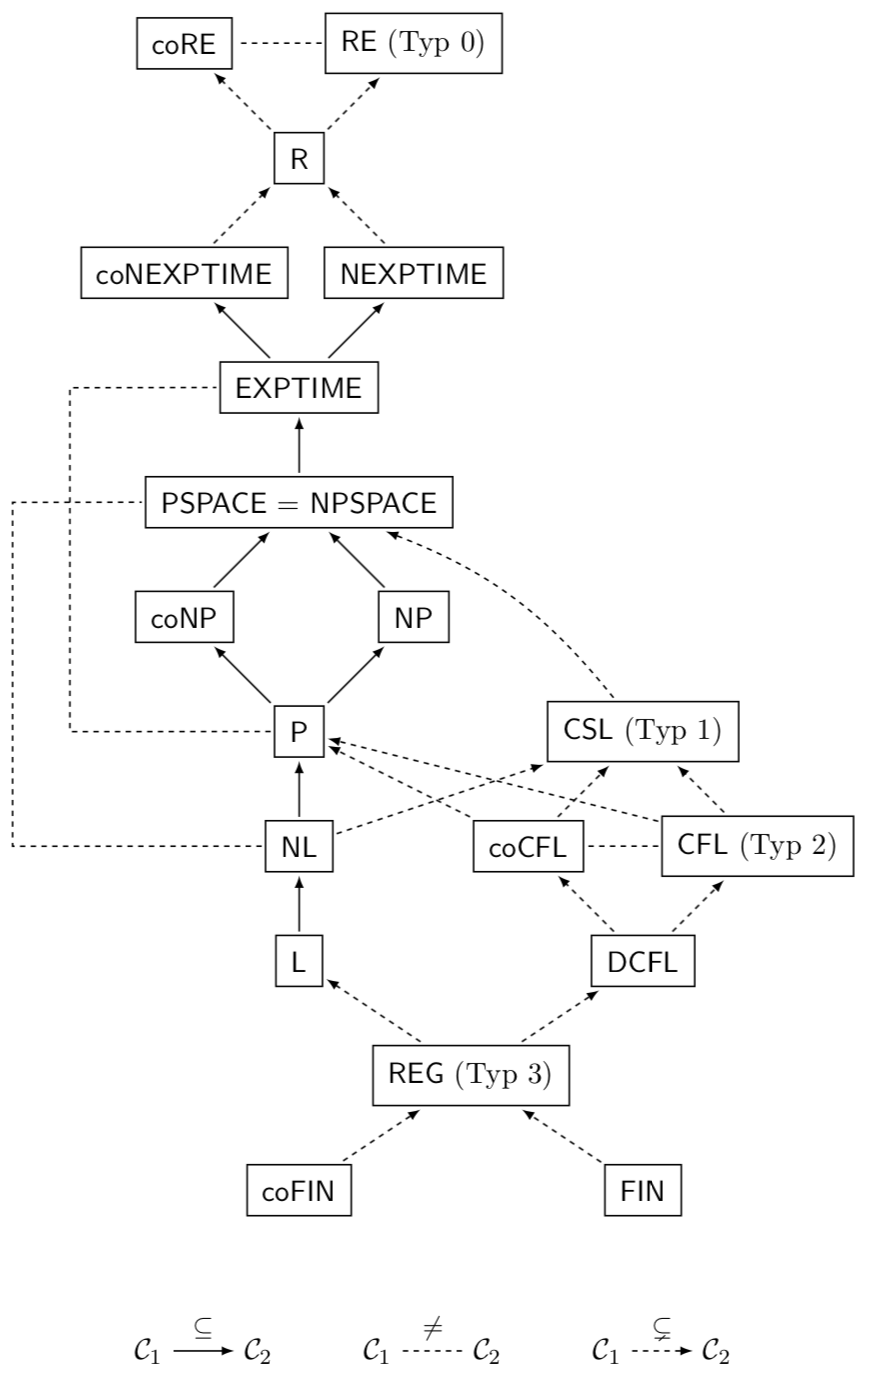
\includegraphics[width=\columnwidth]{graph.png}


	\subsection{Vollständige Probleme}
	\begin{itemize}
		\item Folgende Probleme sind \npoly-vollständig bezüglich $\leq_p$:
		\begin{tabular}{r|l}
			\textbf{SAT} & $\set{w}{w\text{ kodiert eine erfüllbare Formel}}$\\
			\textbf{3KNF-SAT} & KNF mit max. 3 Literalen pro Klausel erfüllbar?\\
			\textbf{CLIQUE} & Enthält ein Graph eine Clique der Größe $k$?\\
			\textbf{FÄRB.} & Gibt es eine Knotenfärbung mit $k$ Farben?\\
		\end{tabular}

		\item \textbf{QBF} ist \textbf{PSPACE}-vollständig.

		\item \poly-vollständig bezüglich $\leq_{\log}$ ist
		\begin{enumerate}
			\item \textbf{CVP}: Circuit Value Problem, Wert eines Schaltnetzes bestimmen
			\item \textbf{$L_{cfe}$}: Leerheit kontextfreier Sprachen
		\end{enumerate}

		\item \textbf{NL}-vollständig bezüglich $\leq_{\log}$ ist
		\begin{enumerate}
			\item \textbf{GAP}: existiert ein Pfad vom source-Knoten zum target-Knoten in einem gerichteten Graphen?
			\item \textbf{2KNF-SAT}
		\end{enumerate}
	\end{itemize}





	\section{Beispiele}
	\begin{itemize}
		\item Verhältnis von $\operatorname{NSPACE}(2^n)$ und $\operatorname{DSPACE}(5^n)$:
		\begin{align*}
			\operatorname{NSPACE}(2^n)\overset{\text{S.v.S.}}\subseteq\operatorname{DSPACE}(2^{2n})\\
			=\operatorname{DSPACE}(4^n)\overset{\text{P.H.S.}}\subsetneq\operatorname{DSPACE}(5^n)
		\end{align*}
		\item \textbf{Folgerung mit Translationssatz}, $\poly\subseteq\textbf{L}\Rightarrow \textbf{EXPTIME}\subseteq\textbf{PSPACE}$:

		Sei $L\in\textbf{EXPTIME}\Rightarrow L\in \operatorname{DTIME}(2^{n^k})$ für ein $k\in\N$, dann ist mit der Translationsfunktion $f(n)=2^{\frac{n^k}{k}}$ (denn $f(n^k)=2^{k*(n^k)*\frac1k}=2^{n^k}$) nach dem Translationssatz für Zeitklassen $Pad_f(L)\in\operatorname{DTIME}(n^k)$.
		Nach der Annahme $\poly\subseteq\textbf{L}$ folgt dann, $Pad_f(L)\in\operatorname{DSPACE}(\log n)$.
		Mit dem Translationssatz für Platzklassen und der selben Funktion folgt, $L\in \operatorname{DSPACE}(\log f(n))=\operatorname{DSPACE}(\log (2^{\frac{n^k}{k}}))=\operatorname{DSPACE}(\frac{n^k}{k})\subseteq\textbf{PSPACE}$.\hfill$\Box$

		\item \textbf{Ungleichheit mit dem Translationssatz}, $\forall c\in\N: \operatorname{NSPACE}(n^c)\neq \npoly$:

		Annahme: $\exists c\in\N: \operatorname{NSPACE}(n^c)=\npoly$. Sei $L\in\operatorname{NSPACE}(n^{3c})$ beliebig. Mit $f(n)=n^3$ folgt dann, $Pad_f(L)\in\operatorname{NSPACE}(n^c)\subseteq\npoly$ nach Annahme. Es existiert also ein $k\in\N: Pad_f(L)\in\operatorname{NTIME}(n^k)$, nach Translationssatz ist $L\in \operatorname{NTIME}(n^{3k})$. Es wurde gezeigt:
		\begin{equation*}
			\operatorname{NSPACE}(n^c)\subseteq\npoly\Rightarrow\operatorname{NSPACE}(n^{3c})\subseteq\npoly
		\end{equation*}
		Damit folgt aber nach Annahme
		\begin{equation*}
			\operatorname{NSPACE}(n^{3c})\subseteq\npoly =\operatorname{NSPACE}(n^c)
		\end{equation*}
		Was im Widerspruch zum Platzhierarchiesatz steht.\hfill$\Box$
	\end{itemize}

\end{multicols}
\end{document}
